\section{\texorpdfstring{AutoLibra as a lens

\includegraphics[height=1em]{figs/microscope.png}
: agent evaluation with AutoLibra}{AutoLibra as a lens: agent evaluation with AutoLibra}}
\label{sec:lens}

In this section, we use AutoLibra as a lens to provide grounded, behavior-salient
insights into agent trajectories. In three data sets, CoGym \citep{shao2024collaborative},
Sotopia \citep{zhousotopia}, and WebVoyager \citep{he2024webvoyager}, we compare
induced metrics with heuristically proposed evaluation dimensions and failure modes
summarized by the authors. We find that AutoLibra can discover more concrete
metrics than heuristically defined categories, and novel metrics that are overlooked
by experts. Tab. \ref{tab:merged_comparison} summarizes the comparison between AutoLibra-induced
metrics and evaluation criteria across the three aforementioned datasets.

% Define colors for matching categories
\definecolor{comm}{RGB}{230,242,255}
\definecolor{sit}{RGB}{255,240,230}
\definecolor{plan}{RGB}{230,255,230}
\definecolor{env}{RGB}{255,230,255}
\definecolor{pers}{RGB}{255,255,230}
\definecolor{goal}{RGB}{242,242,255}
\definecolor{believ}{RGB}{255,242,242}
\definecolor{navstuck}{RGB}{242,255,242}
\definecolor{hall}{RGB}{255,242,255}
\definecolor{misalign}{RGB}{245,245,230}
\definecolor{unmatched}{RGB}{240,240,240}

\begin{table}[!t]
	\centering
	\renewcommand{\arraystretch}{1.2} % Increase row height
	\begin{tabular}{@{}lp{\dimexpr0.50\textwidth}p{\dimexpr0.40\textwidth}@{}}
		\toprule                                                                                          & \textbf{AutoLibra\protect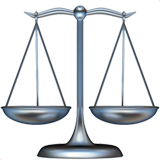
\includegraphics[height=1em]{figs/scale.png}-induced metrics}                                                                                                                                                        & \textbf{Failure categories by experts}                                    \\
		\midrule \multirow{11}{*}{\rotatebox[origin=c]{90}{\textbf{CoGym} \citep{shao2024collaborative}}} & \multicolumn{2}{c}{Matched metrics and failure categories}                                                                                                                                                                                     \\
		\cmidrule(lr){2-3}                                                                                & \cellcolor{comm}\textit{Responsiveness and Efficiency} (75\%)                                                                                                                                                                                 & \cellcolor{comm}                                                          \\
		                                                                                                  & \cellcolor{comm}\textit{Communication Clarity \& Notification} (8\%)                                                                                                                                                                          & \multirow{-2}{*}{\cellcolor{comm}\textit{Communication} (65\%)}           \\
		                                                                                                  & \cellcolor{sit}\textit{Instruction Adherence \& Follow-Through} (24\%)                                                                                                                                                                        & \cellcolor{sit}\textit{Situational Awareness} (40\%)                      \\
		                                                                                                  & \cellcolor{plan}\textit{Iterative Refinement and Adaptability} (47\%)                                                                                                                                                                         & \cellcolor{plan}                                                          \\
		                                                                                                  & \cellcolor{plan}\textit{Autonomy and Proactiveness} (28\%)                                                                                                                                                                                    & \multirow{-2}{*}{\cellcolor{plan}\textit{Planning} (39\%)}                \\
		                                                                                                  & \cellcolor{env}\textit{Content Quality and Coherence} (16\%)                                                                                                                                                                                  & \cellcolor{env}                                                           \\
		                                                                                                  & \cellcolor{env}\textit{Search and Retrieval Accuracy} (13\%)                                                                                                                                                                                  & \cellcolor{env}                                                           \\
		                                                                                                  & \cellcolor{env}\textit{Data Analysis Competence} (2\%)                                                                                                                                                                                        & \multirow{-3}{*}{ \cellcolor{env}\textit{Environmental Awareness} (28\%)} \\
		                                                                                                  & \cellcolor{pers}\textit{Interface and User Experience} (23\%)                                                                                                                                                                                 & \cellcolor{pers}\textit{Personalization} (16\%)                           \\
		\midrule \multirow{13}{*}{\rotatebox[origin=c]{90}{\textbf{Sotopia} \citep{zhousotopia}}}         & \multicolumn{2}{c}{Matched metrics and social dimensions}                                                                                                                                                                                      \\
		\cmidrule(lr){2-3}                                                                                & \cellcolor{goal}\textit{Goal Achievement \& Outcome Effectiveness} (19\%)                                                                                                                                                                     & \cellcolor{goal}\textit{Goal Completion} (14\%)                           \\
		                                                                                                  & \cellcolor{believ}\textit{Conversational Naturalness \& Efficiency} (5\%)                                                                                                                                                                     & \cellcolor{believ}                                                        \\
		                                                                                                  & \cellcolor{believ}\textit{Personality Consistency and Alignment} (2\%)                                                                                                                                                                        & \cellcolor{believ}                                                        \\
		                                                                                                  & \cellcolor{believ}\textit{Contextual Integration of Identity} (1\%)                                                                                                                                                                           & \multirow{-3}{*}{\cellcolor{believ}\textit{Believability} (4\%)}          \\
		\cmidrule(lr){2-3}                                                                                & \multicolumn{2}{c}{Unmatched AutoLibra\protect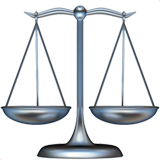
\includegraphics[height=1em]{figs/scale.png}-induced metrics}                                                                                                                                    \\
		\cmidrule(lr){2-3}                                                                                & \multicolumn{2}{C{0.93\textwidth}}{\cellcolor{unmatched}\textit{Negotiation Tactics and Strategic Adaptability} (14\%), \textit{Responsiveness and Conversational Termination} (5\%), \textit{Adaptability and Flexibility in Dialogue} (7\%)} \\
		\cmidrule(lr){2-3}                                                                                & \multicolumn{2}{c}{Unmatched Sotopia-Eval dimensions}                                                                                                                                                                                          \\
		\cmidrule(lr){2-3}                                                                                & \multicolumn{2}{C{0.93\textwidth}}{\cellcolor{unmatched}\textit{Relationship, Knowledge, Secret, Financial and Material Benefits, Social Rules}}                                                                                               \\
		\midrule \multirow{14}{*}{\rotatebox[origin=c]{90}{\textbf{WebVoyager} \citep{he2024webvoyager}}} & \multicolumn{2}{c}{Matched metrics and failure reasons}                                                                                                                                                                                        \\
		\cmidrule(lr){2-3}                                                                                & \cellcolor{navstuck}\textit{Error Recovery \& Adjustment} (15\%)                                                                                                                                                                              & \cellcolor{navstuck}                                                      \\
		                                                                                                  & \cellcolor{navstuck}\textit{Step Efficiency \& Action Redundancy} (13\%)                                                                                                                                                                      & \cellcolor{navstuck}                                                      \\
		                                                                                                  & \cellcolor{navstuck}\textit{Navigation Accuracy} (11\%)                                                                                                                                                                                       & \cellcolor{navstuck}                                                      \\
		                                                                                                  & \cellcolor{navstuck}\textit{Access Barrier Handling} (2\%)                                                                                                                                                                                    & \multirow{-4}{*}{\cellcolor{navstuck}\textit{Navigation Stuck} (44\%)}    \\
		                                                                                                  & \cellcolor{hall}\textit{Information \& Verification Accuracy} (16\%)                                                                                                                                                                          & \cellcolor{hall}\textit{Hallucination} (22\%)                             \\
		                                                                                                  & \cellcolor{misalign}\textit{Result Relevance Accuracy} (9\%)                                                                                                                                                                                  & \cellcolor{misalign}\textit{Prompt Misalignment} (9\%)                    \\
		\cmidrule(lr){2-3}                                                                                & \multicolumn{2}{c}{Unmatched AutoLibra\protect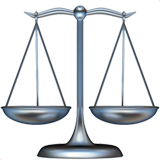
\includegraphics[height=1em]{figs/scale.png}-induced metrics}                                                                                                                                    \\
		\cmidrule(lr){2-3}                                                                                & \multicolumn{2}{C{0.93\textwidth}}{\cellcolor{unmatched}\textit{Query and Search Strategy Efficiency} (7\%), \textit{Final Output and Summarization Quality} (18\%)}                                                                           \\
		\cmidrule(lr){2-3}                                                                                & \multicolumn{2}{c}{Unmatched WebVoyager fail reasons}                                                                                                                                                                                          \\
		\cmidrule(lr){2-3}                                                                                & \multicolumn{2}{C{0.93\textwidth}}{\cellcolor{unmatched}\textit{Visual Grounding Issue} (25\%)}                                                                                                                                                \\
		\bottomrule
	\end{tabular}
	\caption{Comparison between AutoLibra-induced metrics and expert proposed
	evaluation dimensions and failure categories. The percentages in parenthesis denote
	frequency of -1 in AutoLibra-induced metrics, and failure frequency or score from
	the original papers.}
	\label{tab:merged_comparison}
	\vspace{-20pt}
\end{table}

\paragraph{CoGym}
For CoGym \citep{shao2024collaborative}, AutoLibra induces 9 metrics from
feedback from \textbf{end users}, which can correspond to the five failure
categories proposed by the authors. The failure rate (frequency of a metric
score of -1) measured by AutoLibra also roughly matches the failure rate of the
manually labeled CoGym categories by the authors. This shows that AutoLibra induces
metrics that reflect human-expert categorization and provide an automated measurement
of agent failures.

%\textit{Communication clarity and user interaction} belongs to Communication,  \textit{Adherence to instructions and consistency} belongs to Situational Awareness, \textit{Adaptability and responsiveness to feedback} belongs to Planning, \textit{Search accuracy and content relevance} belongs to Environment Awareness, and \textit{User preference query and incorporation} belongs to Personalization. All five metrics are more concrete and fine-grained than the larger categories in CoGym; we also discover the following metrics that are not mentioned in the break-down analysis in the CoGym paper:
%\textit{Responsiveness and Efficiency}, \textit{Content Quality and Coherence}, and \textit{Data Analysis Competence}. We note that this comparison shows the complementary characteristics of automatically
%induced metrics, which are more concrete on the issues that users are noticing, while the expert-designed categories measure the high-level capabilities of AI agents.

\paragraph{Sotopia}
Sotopia \citep{zhousotopia} proposed 7 dimensions for evaluating
social intelligence in AI agents. With AutoLibra, we recover the exact dimension
\emph{Goal Completion}, and 3 metrics as the subdimensions of \emph{Believability},
indicating that \textit{Believability} could be too high-level, while AutoLibra provides
more concrete breakdown metrics. The failure rate (frequency of a score of -1
metric rating, indicating the agent performs poorly on that metric) measured by
AutoLibra in these two categories roughly matches the score of the Sotopia
dimensions of the agent we studied. AutoLibra induces another four metrics 
overlooked in the heuristically proposed Sotopia-Eval dimensions. We note that
the other five dimensions in Sotopia are still valuable evaluation dimensions
for social intelligence. However, behaviors captured by dimensions \emph{Financial
and Material Benefits}, \emph{Knowledge}, and \emph{Secret} are often also captured
by \textit{Goal Completion} and \textit{Believability}. As a result, AutoLibra produces
the single \textit{Goal Achievement and Outcome Effectiveness} by minimizing
redundancy. Whereas, \textit{Relationship} and \textit{Social Rules} captures
long-tailed behaviors not captured by AutoLibra.

\paragraph{WebVoyager}
Similarly, for web navigation tasks, AutoLibra also discovers metrics such as \textit{Access
Barrier Handling}, \textit{Error Recovery and Adjustment}, \textit{Step
Efficiency and Action Redundancy}, and \textit{Navigation Accuracy}, which much more
closely reflect concrete agent behavior than the failure analysis categories proposed
in previous work \citep{he2024webvoyager,zhou2024proposeragentevaluatorpaeautonomousskilldiscovery},
where they are often simply classified as ``navigation stuck''. We also find
additional metrics that are not mentioned in the failure analysis, such as \textit{Query
and Search Strategy Efficiency} and \textit{Final Output and Summarization
Quality}, which are frequent issues (with frequencies of 7\% and 18\%). Since AutoLibra
only observes the behavior of the agents, it cannot interpret the neural
representation, not able to capture the visual grounding issues, which are
mentioned in the WebVoyager paper. This further demonstrates AutoLibra's utility
in extracting behavior-salient metrics, and particularly its
ability to obtain \textbf{fine-grained metrics} that expert design would not have
been able to extract.